\begin{figure}
	\tikzsetnextfilename{gauss-green-normale-x}
	\centering
	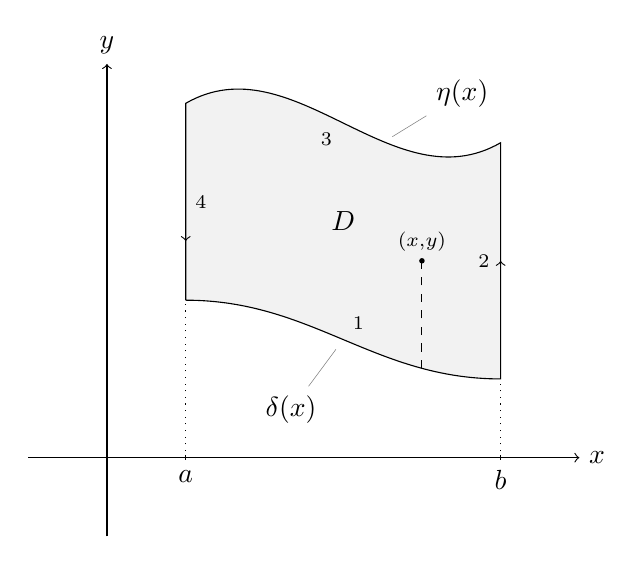
\begin{tikzpicture}
		\draw [black,->] (-1,0) -- (6,0) node[right]{$x$};
		\draw [black,->] (0,-1) -- (0,5) node[above]{$y$};
		\fill [black!5!white] (1,2) to[out=0,in=180] (5,1) -- (5,4) to[out=210,in=30] (1,4.5) -- cycle;
		% \fill va prima del disegno del contorno, altrimenti si sovrappone a tutto e lo nasconde
		\draw [black] (1,2) to[out=0,in=180] node[auto]{$\vgamma_1$} (5,1)
			to node[auto]{$\vgamma_2$} (5,4)
			to[out=210,in=30] node[auto]{$\vgamma_3$} (1,4.5)
			to node[auto]{$\vgamma_4$} (1,2);
		\draw [dotted] (1,0) -- (1,2);
		\draw [dotted] (5,0) -- (5,1);
		\node [pin={[pin distance=5mm]250:{$\delta(x)$}}] at (3,1.5) {};
		\node [pin={[pin distance=5mm]30:{$\eta(x)$}}] at (3.5,4) {};
		\node at (3,3) {$D$};
		% Dato che non TikZ non ha un comando per disegnare frecce in mezzo alla linea, mi devo arrangiare.
		% Traccio nuovamente le linee del bordo dell'insieme fino a -- più o meno -- metà, mettendo una freccia sulla
		% punta a queste. Non le disegno sui tratti curvi perche' sarebbe troppo complicato: dovrei spezzare in due anche
		% la linea tracciata prima con \draw (l. 10 e segg.) ma allora l'etichetta con il nome \vgamma del tratto non
		% risulterebbe più centrata.
		\draw [black,->] (1,4.5) -- (1,2.75); 
		\draw [black,->] (5,1) -- (5,2.5);
		% Queste sono le tacche sull'asse x in corrispondenza delle due linee tratteggiate in x=a e x=b
		\draw (1,1pt) -- (1,-1pt) node[below]{$a$};
		\draw (5,1pt) -- (5,-1pt) node[below]{$b$};
		% Questa è la curva che congiunge l'angolo (a,\delta(a)) in basso a sinistra del bordo con un punto generico nell'insieme.
		% È disegnata per ultima in modo che non sia nascosta da niente.
		% L'angolo di entrata ('in') è una combinazione di fortuna e tanta pazienza: purtroppo non so un modo per calcolarlo
		% automaticamente...
		\draw[black,dashed] (4,1.135) -- (4,2.5) node[above]{$\scriptstyle(x,y)$};
		\fill[black] (4,2.5) circle (1pt);
	\end{tikzpicture}
	\caption{Parametrizzazione del contorno di un dominio $D$ come nel punto (ii) della dimostrazione del teorema \ref{t:gauss-green} di Gauss-Green.}
	\label{fig:gauss-green-normale-x}
\end{figure}
